\section{Using what we have seen so far}
\begin{frame}{Steps}
	\begin{itemize}
		\item Settle on a class of function with parameters  to be optimized. 
		 
		\item Define a secondary function - the loss function.  
		 
		\item Split data into  training set, validation set and test 
		set. Use randomization. For the following discussion, we ignore validation set. 
		
		\item Initialize model weights (W's or $\theta$s), typically using 
		small random numbers.
	  
		\item Iterate over the data in batches  
		\begin{itemize}
			\item compute the predicted value
			\item compute the loss 
			\item compute gradients 
			\item update parameters
		\end{itemize}
		\item Keep track of loss and stop when loss stops decreasing.
		\item Compute loss for test set.   
	\end{itemize}
\end{frame}

\begin{frame}{Python code}
		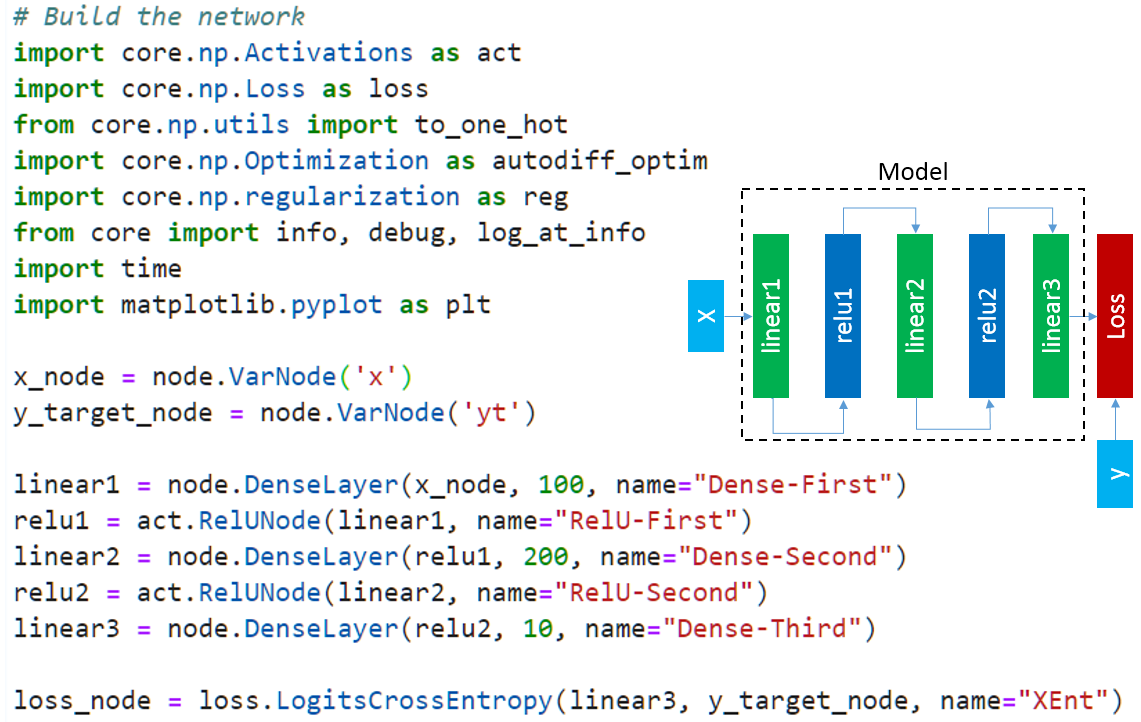
\includegraphics[width=.9\textwidth, center]{figuras/3layer_autodiff_example_with_network.png}	
\end{frame}

\begin{frame}{Learning, libraries etc.}
\begin{block}{Libraries}
	\begin{itemize}
		\item Torch and Theano 
		\item Tensorflow  
		\item Keras
		\item Pytorch  
	\end{itemize}	
\end{block}

\begin{block}{Recommendations for those just starting}
	\begin{enumerate}
		\item Build from scratch using numpy 
		\begin{itemize}
			\item Linear/Dense 
			\item Optimization,  Regularization,  Activations 
			\item Basic CNN and RNN
		\end{itemize} 
		\item Pytorch  
	\end{enumerate}	
\end{block}
\end{frame}

\begin{frame}{Next}
	\begin{block}{Part II}
		\begin{itemize}
			\item Autoencoders and PCA 
			\item Convolution neural networks 
			\item Recurrent neural networks 
			\item Transfer learning 
			\item GANs (possibly!) 
		\end{itemize}		
	\end{block}

\end{frame}
